\documentclass[a4paper,11pt]{exam}
    \usepackage{hyperref}
    \ifx\pdftexversion\undefined
       \usepackage{epsfig}
    \else
       \usepackage[pdftex]{graphics}
    \fi
    \usepackage{epsfig}
    \usepackage{verbatim}
\begin{document}
    \extraheadheight{.5in}
    \firstpageheader{\large\sf CS2105}%
    {\large\sf National University of Singapore\\ School of Computing \\
    \LARGE\sf Assignment 1}%
    {\large\sf Semester 2 13/14}
    \firstpageheadrule
    \pagestyle{headandfoot}

    \section*{Deadline}

    21 February, 2014 (Friday), 11:59pm.

    \section*{Objective}

    In this assignment, you will learn how a Web application works. In particular, you will see how a Web client communicates with a Web-based application using Common Gateway Interface (CGI) through a Web server.

    \section*{Pre-requisite}

You are expected to know the format of HTTP request and response messages, socket programming with TCP, and how to write a simple Web server that supports GET. 

    The assignment will be done under a controlled UNIX environment. Familiarity with UNIX environment (how to copy/move/delete/edit files, how to compile and run programs, etc.) is assumed.

    You should use Chrome version 32 or above as your Web client for this assignment.  You may additionally choose to support other browsers.  The ``Developer Tools'' for Chrome might be useful for debugging.

    \section*{Administrative Matters}

This is a 2-person team assignment.  

An account has been set up for each student in class on host cs2105-z.comp.nus.edu.sg. To access your account, ssh to the host and login using your SoC UNIX username and password \textit{from a SoC host or through SoC VPN}.

If you have any question or encounter any problem with the steps discussed in the assignment, please contact the teaching staff through CS2105's blog.

\section*{Background}

In the early days of the World Wide Web, the Web consists only of static Web pages. Web clients send HTTP requests to Web servers, which then read the requested Web objects (HTML files, images) and return them to the Web clients in a HTTP response message.

Soon, people realize that the Web can be much more powerful -- by allowing the Web server to interface with back-end applications, users can use the Web to access and store information on remote applications the same way they have been doing using applications on their local machines. This new way of interacting with remote applications enables Web-based applications (Facebook, Gmail, IVLE, CORS etc.). The Web server can be viewed as a gateway to these back-end applications. A standard called Common Gateway Interface, or CGI, was established to define how the client, the server, and the back-end applications (also termed CGI scripts) communicate (See Figure 1).

The Web server's responsibilities include (i) receive the HTTP request from the client, (ii) decide which CGI script to handle the client's request based on the URI supplied by the client, (iii) transform the client request into a CGI request, (iv) execute the CGI script, and (v) convert the CGI response into a response for the client.

\begin{figure}
\begin{center}
	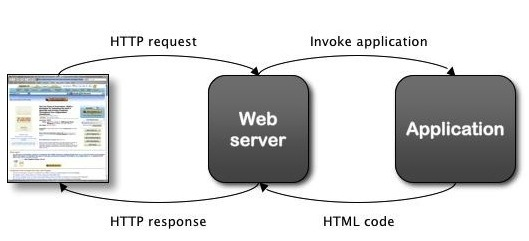
\includegraphics[width=0.7\textwidth]{cgi.jpg}
\end{center}
\caption{Communication between Web client, server, and back-end application.}
\end{figure}

Scripting languages such as Perl was a popular choice for writing CGI scripts. Several frameworks, such as ASP, JSP, PHP, ColdFusion, Ruby on Rails, were later developed to provide rapid web application development with better support for templating HTML code and database access. Modern Web servers commonly integrate interpreter of these languages into the Web servers to improve performance.

\section*{Your Tasks}

In this assignment, you will modify the simple Web server given in class to interface between Web clients and a given CGI script. To simplify the assignment, you are not expected to fully implement the HTTP and CGI standard as specified in the RFCs, but only enough for the given CGI scripts to function. The details of what your Web server should support and some Java tips on how you can do it is given below.

\textit{You only need to support HTTP 1.0 for this assignment.}

\subsection*{Processing HTTP Requests}

    The given Web server can already read HTTP requests from the client. Your Web server, however, should distinguish between different types of HTTP requests. For this assignment, we are interested in GET and POST methods. The given code supports only HTTP GET on static files. Web servers are typically configured to recognize static files through file extensions. Common static file extensions are gif, jpg, htm, html, etc., whereas dynamic Web pages can have extensions such as php, cgi, asp. For this assignment, the only file extension for dynamic Web pages you need to recognize is ``.pl'' (for Perl scripts).  When the requested file has an extension of ``.pl'', your Web server shall execute the Perl script (more on this later) instead of sending the content of the Perl script back to the client.

	When the client uses GET to retrieve a static file, your Web server should send the requested file back to the client as shown in the lecture.  You need to send back the appropriate ``Content-Type'' header depending on the file type.  For the list of content types, see \url{http://www.iana.org/assignments/media-types}.

    When the client uses GET to invoke a CGI script, the URL may encode additional arguments for the CGI script. Such "script URL" typically looks like this:

\begin{verbatim}
http://www.google.com.sg/search?hl=en&q=CS2105+Networks&meta=
\end{verbatim}

    In the example above, search refers to the script that the server should run. The arguments to the script (e.g., what to search?) are given in the format of key=value. The ampersand \& separates the key-value pairs, and the question mark ? separates the name of the script with the arguments.

    Note that a value can be empty, and the arguments may need to be encoded due to restrictions on URL format. For instance, a plus ``+'' in the URL above represents a white space. This encoding is called URL encoding. You are not required to decode URL encoded strings in this assignment.

    The section of a script URL after the question mark is called query string. The query string is one method a Web client can send information to the server.

    The other HTTP method we are interested in is the HTTP POST method. There are two forms of POST requests -- differentiated by their ``content type''. To determine the content type of a POST request, you should look at the ``Content-Type:'' line of the HTTP request header.

    The first content type is \texttt{application/x-www-form-urlencoded}. This type of POST request is not much different from GET request. The only difference is that the query string, instead of becoming part of the URL, is stored in the body of the HTTP request.

    Using query strings to pass information from the client to the server has its limitation. An example is when the client needs to upload a file to the Web server (e.g., uploading a file to IVLE Workbins). It is not feasible to encode the whole file inside the query string. For this reason, there exists a second way of encoding information in a POST request.

    The second content type is called \texttt{multipart/form-data}. Instead of using key-value pairs to encode information, the body of the HTTP POST request looks something like this:

    \begin{verbatim}
Content-Type: multipart/form-data; boundary=LKJhl876x

--LKJhl876x
Content-Disposition: form-data; name="q"

CS2105 Networks
--LKJhl876x
Content-Disposition: form-data; name="files"; filename="file1.txt"
Content-Type: text/plain

... contents of file1.txt ...
--LKJhl876x--

\end{verbatim}

Since you are not required to parse the HTTP POST body, I will not go into details about the format above.

\subsection*{CGI scripts and CGI requests}

Once your Web server receives the HTTP requests (regardless of POST or GET) for a CGI script, your Web server should execute the script and pass the necessary information (e.g. query strings, uploaded files) to the script for processing. This section explains how your Web server can do that.

There are two ways the Web server communicates with a CGI script. The first method is through environment variables. (See Wikipedia's entry on environment variables if you are not familiar with this term.) The CGI standards called these environment variables \textit{meta-variables}. According to the standards, there are many meta-variables that should, or must, be set for CGI scripts to run properly. For the purpose of this assignment, we are only interested in four environment variables: REQUEST\_METHOD, QUERY\_STRING, CONTENT\_TYPE, and CONTENT\_LENGTH. The Web server sets the environment variables to proper values before calling the CGI script. When invoked, the CGI script reads the value of the environment variables.

The second method to communicate with a CGI script is by writing directly into its standard input. When HTTP POST method is used, the CGI script expects to read data from its standard input. By writing the data to the script standard input, the Web server can pass the data to the script.

Which methods to use and which variables to set depend on the HTTP method. The environment variable that you always have to set is REQUEST\_METHOD. Your Web server should always set REQUEST\_METHOD to either POST or GET, depending on the HTTP request received. If the REQUEST\_METHOD is GET, your Web server should set QUERY\_STRING to the query string of the HTTP request. Remember to set the QUERY\_STRING to empty when there is no query string in the URL.

When HTTP POST request is received, your Web server must set CONTENT\_TYPE and CONTENT\_LENGTH to their appropriate values according to the HTTP request header, and then write the HTTP body of the POST request to the standard input of the CGI script. It is important to set the CONTENT\_LENGTH correctly and send the corresponding number of bytes to the CGI script.

\subsection*{Output from CGI scripts}

The CGI script prints its data to its standard output. The Web server can use a pipe to read its data. Your server should send the data (by prefix it with correct HTTP response code) back to the client.

For debugging purposes, it would be useful for your Web server to read from the standard error of the CGI scripts, and print the error messages to its own standard output/error.

Note that we will ignore standard error and standard output from your Web server during grading.

\section*{Your Web Application: To-Do List}

In this assignment, you will be given two CGI scripts, one is for debugging purposes, and the other implements a simple web-based to-do list. This application allows user to add and delete to-do items. Each item has an associated description. You can add additional notes to each item. The notes can be edited. The rest of this section describes the functionality of this web application.

\begin{figure}
\begin{center}
	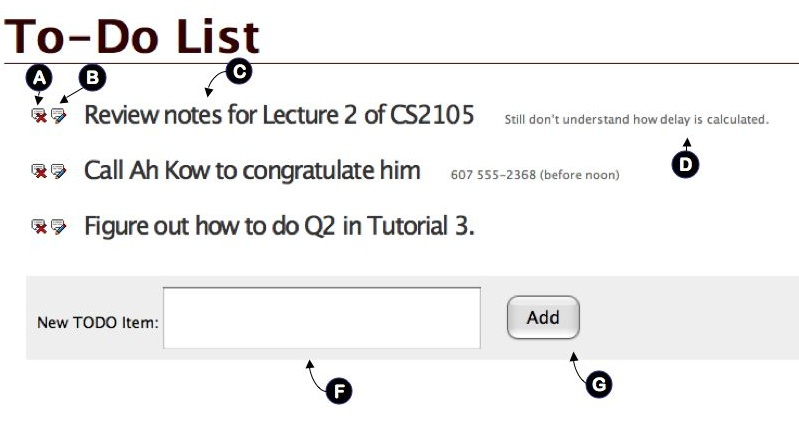
\includegraphics[width=0.8\textwidth]{todo-list.jpg}
\end{center}
\caption{To-Do List Interface}
\end{figure}

Figure 2 shows a screen shot of the to-do list application. The important elements of the user interface are labeled from A to G:

\begin{itemize}
	\item A: Delete button. Click to delete the current to-do item, including description and notes.
	\item B: Edit button. Click to edit the current to-do item, including description and notes. (it will bring the user to the next screen).
	\item C: Description. A short string describing the to-do item. Cannot be empty.
	\item D: Notes. Optional note pertaining to the corresponding to-do item.
	\item F: Input textbox . Enter the description of a new to-do item.
	\item G: Add button. Add a new to-do item with the current description entered in the textbox.
\end{itemize}

\begin{figure}
\begin{center}
	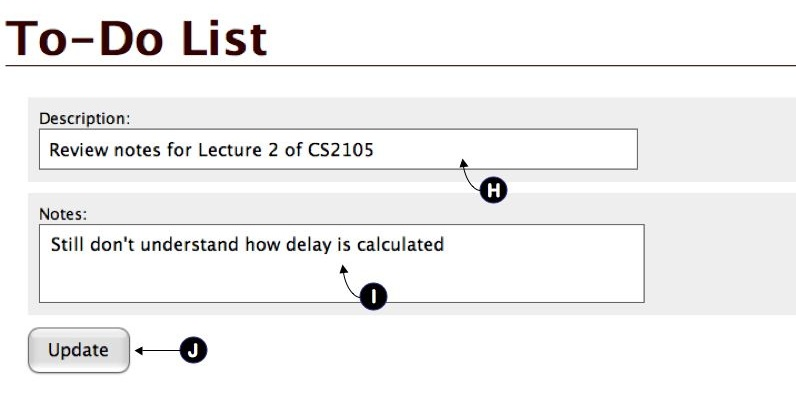
\includegraphics[width=0.8\textwidth]{todo-edit.jpg}
\end{center}
\caption{To-Do List Interface}
\end{figure}

Figure 3 shows the screen when the edit button (B) is pressed.


The following are the user interface elements on screen.

\begin{itemize}
	\item H: A textbox to edit the description of the to-do item.
	\item I: A textbox to edit the notes of the to-do item.
	\item J: Update button -- when click, the descriptions and notes will be updated. After the user clicks ``update'', the updated to-do list will be shown as in the previous screen.
\end{itemize}

\section*{How HTTP Requests Are Generated}

The todo application is implemented in the script todo.pl. Calling todo.pl directly (using GET without any query string) would generate a list of to-do items. Clicking on button A and B would generate a GET request with appropriate query strings. Clicking on G generates a POST request with content type application/x-www-form-urlencoded. Finally, clicking on J generates a POST request with content type multipart/form-data.

(It might be easier to implement the features of your Web server incrementally in the order explained in the previous paragraph.)

\section*{How to Do It in Java}

\subsection*{Calling an external program}

You can use the exec() method of the Runtime class in Java to execute an external program. To execute a CGI script written in Perl, e.g. /home/o/ooiwt/a1/todo.pl, you can use the following code\footnote{Of course, you should not hardcode the paths in your code, as in this example.}:

\begin{verbatim}
Runtime.getRuntime().exec("/usr/bin/perl /home/o/ooiwt/a1/todo.pl");
\end{verbatim}

The call returns a Process object. You will need to use the Process object later.

\subsection*{Setting Environment Variables}

You can set a series of environment variables in UNIX using the command env. From the UNIX command line, you can use env to modify the environment variables before calling another program as follows.

\begin{verbatim}
/usr/bin/env KEY1=value1 KEY2=value2 program
\end{verbatim}

The command above executes \texttt{program} AND sets the environment variables \texttt{KEY1} and \texttt{KEY2} for the process associated with \texttt{program}.  The environment variables set are not persistent, i.e., they will be cleared after the process ends.

To set the environment variables before calling a CGI script within Java, you can use the exec() method of Runtime class just like before.

\subsection*{Reading and Writing to a Process}

The exec() method of Runtime class returns a Process object. To read and write to the process, you need a handle to the input stream and output stream of the process. This is similar to the input stream and output stream of a socket and can be used in exactly the same way (using BufferedReader to read and DataOutputStream to write).

For example, to send the string "hello" to the standard input of some process p,

\begin{verbatim}
DataOutputStream o = new DataOutputStream(p.getOutputStream());
o.writeBytes("hello");
\end{verbatim}

\section*{Your cs2105-z Account}

An account on the server, cs2105-z.comp.nus.edu.sg, has been setup for you. From within SoC (or through SoC-VPN), ssh to cs2105-z using your SoC UNIX id and password.

Copy the files prepared for you to your home directory, by executing:

\begin{verbatim}
cp -r ~sadm/a1 .
\end{verbatim}

You will see the following files:

\begin{itemize}
	\item todo.pl -- Perl script that implements the to-do list application.
	\item debug.pl -- Perl script to help you debug.
	\item TODO and data -- file-based database to store to-do list items. If you found that the database is corrupted, simply remove all contents from the file TODO and the directory data to restart all over again.
	\item edit.gif, del.gif, style.css -- images and style file used by the to-do list application.
\end{itemize}

Note that you must put your files inside the directory \texttt{a1} directly under your home directory (i.e., \texttt{\$HOME/a1}). This is the root of your Web directory.  

\textit{You should ensure that the files in the directory of both team members are updated to the latest version before the deadline.  We will randomly pick the files from one of the team member to grade.}

\subsection*{File Permission}

You will be responsible for the security of your own source code. Please be careful and set the correct permission for your files. They should not be readable by anyone else except the owner (chmod 600 *.java will ensure that).

If you use an online source code repository for revision control, please use a private one.  

\section*{Port Numbers}

Your Web server must listen to a non-standard port number. Once your Web server is up and running, you can connect to it through the Web browser on any SoC machines (or SoC-VPN enabled machine) by specifying the port number as part of the URL. For example, if your Web server is running on port 9090, use http://cs2105-z.comp.nus.edu.sg:9090/todo.pl to access the file todo.pl under your \$HOME/a1 directory. You should, of course, write your Web server in such a way that it reads from \$HOME/a1.

To make it easy to use a different port number, your Web server must take in the port number as a command line argument. For instance, to run your Web server on port 9090,

\begin{verbatim}
java WebServer 9090
\end{verbatim}

Note that all of you will be running your Web server on the same host, and therefore must use a different port number. To prevent collision, you should avoid ``nice'' port numbers such as 8000 or 8080.

If you do not know how to parse command line arguments in Java, take a look at \url{http://docs.oracle.com/javase/tutorial/essential/environment/cmdLineArgs.html}.

\section*{Submission and Grading}

There is no need to submit the program by email or IVLE workbin. We will collect your assignment from your home directory on cs2105-z.comp.nus.edu.sg when the deadline is over.

We will test your assignment automatically using a grading program. For this to work, you must not modify todo.pl in any way. If you suspect that there is a bug in todo.pl, please contact us by commenting on the blog.  In addition, there will be a short demo slot for both team members to explain their program to the teaching staff. 

You MUST name your java program WebServer.java. We will only compile this file when we grade. You MUST not implement additional classes in other *.java files.

\section*{Using Another Platform}

If you like to work on your assignment on other platforms (Windows, Mac) that you are more familiar with, you are free to do so. But when you submit your assignment, you should ensure that your program runs properly under cs2105-z.comp.nus.edu.sg and your WebServer.java is located under \$HOME/a1 on cs2105-z.comp.nus.edu.sg.

\section*{Clean Code}

In the example WebServer.java given, the whole server is (intentionally) written in one main method, to highlight the simplicity of writing a minimal working Web server.

As you will augment this code with much additional functionalities, writing everything in one main function will lead to long, unreadable, unmaintainable code.  You should organize reusable parts of your code into smaller methods.

Other good clean coding practice we will look at:
\begin{itemize}
	\item comments/documentation
	\item consistent naming convention
	\item consistent indentation
	\item avoid hardcoding of paths/port numbers
\end{itemize}

\section*{Common Bugs}

Here are some tips on how to avoid common bugs made by students from previous years.
\begin{itemize}
		\item Do not hard code the name of the scripts -- your Web server should be general and not only used for the TODO application.  So the name of the script should be retrieved from the HTTP request.
		\item Use dynamic size arrays -- if you hardcode your array size with a magic number (say, 10000 bytes), your code will not work when the content being returned is larger than the array size.
		\item Beware of newline characters -- HTTP headers use newline characters as special markers.  If you called \texttt{readline()}, the newline characters are removed!
		\item Make sure you return the correct content type in your HTTP response header (including CSS files).
		\item Beware of duplicate ``Content-Type:'' -- Both todo.pl and debug.pl returns the content type as the first line of the output, so you need not insert another content type.
		\item If you move your code to your teammate's account, make sure that your program is running the perl script from the teammate's directory.
		\item Make sure you handle errors properly, especially failure in reading or running the Perl script.
\end{itemize}

\section*{Plagiarism Warning}

You are free to discuss the assignment with your peers. But, ultimately, you should write your own code. We employ zero-tolerance policy against plagiarism. If you are caught copying from another team, or let another team copies your code, you will receive zero for this assignment. Further disciplinary action may be taken by the school.

Note that copying from students from previous semesters of CS2105 is considered plagiarism as well.

\section*{Grading}

\begin{itemize}
\item 1 mark: Cleanliness of code. 
\item 2 marks: Able to invoke CGI script and return output (when calling todo.pl without query string).
\item 2 marks: Able to handle GET request correctly.
\item 3 marks: Able to handle POST request correctly.
\item 2 marks: Answering questions during demo (individual marks).
\end{itemize}

We \textit{will deduct one mark} for every failure to following instructions (wrong directory name, wrong filename for WebServer.java, not taking in port number as a command line argument, inconsistent copies in the directory of team members, etc.)

\section*{Late Submission}

We deduct one mark for every hour after the submission deadline.  We will use the last modified timestamp on the server as submission time.

\vfill
\center\Huge{THE END}
\end{document}
